%%=========================================
\section[Teori \& Relatert arbeid]{Teori \& Relatert arbeid}
%%=========================================
\subsection{Smarte hjem}
\label{ch:smartehjem}
I introduksjonen definerte jeg smarte hjem til å være boliger der miljøet og apparater kan programmeres og styres. Dette er ikke ny teknologi. Muligheten for å kontrollere hus og hytter på avstand har vært tilgjengelig for de mest interesserte i lang tid. \citet{peine08} viser til at ideén om smarte hjem har vært beskrevet siden 80-tallet, men har i de senere år fått en ny interesse i industrien. Styring i kontorbygninger har eksistert siden 70-tallet, med muligheter for å kontrollere lys, varme, elektrisitet og adgangskontroll fra et sentralt sted. Det tok noen år før man innså at de samme egenskapene kunne være ønskelige i private hjem. Den sentrale forskjellen mellom et vanlig hjem og et smart hjem, er altså denne muligheten til å styre flere aspekter ved hjemmet gjennom en sentral enhet.

På markedet finnes det nå flere løsninger for å automatisere deler av hjemmet eller tilby brukergrensesnitt for å styre funksjonalitet som lys og varme. Disse løsningene bidrar med å ivareta sikkerhet og ved å begrense energiforbruket. Det tilbys gjerne informasjon om hjemmet via en app til smarttelefonen slik at brukeren kan ha oversikten selv når han er bortreist. Ved å installere moderne enheter med internettilknytning, som termostater, lys, låser, sikkerhetssystemer og garasjeporter, kan brukeren avlese informasjon og styre enhetene med smarttelefonen.

Denne neste generasjonen apparater med internettilkobling bringer spennende muligheter, men samtidig utfordringer. \emph{Tingenes internett} spås en enorm vekst de neste årene. Se for deg følgende scenario: alle elektriske enheter og apparater i hjemmet er koblet på nettet, hjemmet har et stort antall internettkoblede sensorer for å måle temperatur, lys, bevegelse og tilstedeværesle, og lys, dører og persienner er også koblet til nettet. Det vil være en utfordring å håndtere alle disse dataene på en ansvarlig måte og å tilby gode måter for å lære om og styre hjemmet.

Det finnes ikke et eget fagområde for smarte hjem. Teknologiene og teknikkene som kan brukes for å skape smarte hjem har tilknytning til en rekke fagområder, som bygningsautomasjon, kybernetikk, nettverk, sikkerhet, human-computer interfaces (HCI), artificial intelligence (AI) og ambient intelligence (AmI).

\emph{AmI} er spesielt interessant i kontekst av smarte hjem fordi det omhandler miljøer som er sensitive og responsive til mennesker. Det er en visjon på hvordan vi bruker teknologi i omgivelsene for å støtte opp under hverdagslige aktiviteter. Ettersom enhetene som utgjør denne teknologien stadig blir mindre og stadig blir bedre på å kommunisere seg i mellom, vil teknologien forsvinne inn i omgivelsene. Det eneste synlige vil være brukergrensesnittet vi har designet for å aktivt interagere med teknologien. Dette er en videreføring av framtidssynet \citet{weiser91} skriver om, der teknologien forsvinner inn i hverdagslivet inntil det er umulig å skille de to. \emph{AmI} omhandler alle miljøer vi befinner oss i og vil dermed også kunne omfatte hjemmet.

For å være til hjelp for oss må hjemmet forstå omgivelsenens tilstand og det vil være nødvendig å analysere sensorinformasjon. Jeg har allerede nevnt enkle sensorer, som temperatur og bevegelse, og i kombinasjon kan disse danne et godt bilde av hva som foregår i hjemmet. To langt mer datarike input-kanaler er lyd og bilde. Ettersom vi mennesker kommuniserer med tale er det kanskje også naturlig at hjemmet skal forstå tale? Talegjenkjenning er et vanskelig problem, men det er et fagområde det er gjort store framskritt i de seneste årene. Jeg vil greie ut om bakgrunnsteorien til talegjenkjenning i det neste delkapittelet. Tilsvarende til tale kan man få en datamaskin til å forstå visuell input gjennom kameraer. \citet{augustonugent06} omtaler datasyn som svært nyttig for å gjenkjenne mønstre i menneskers oppførsel eller oppdage når noe galt har skjedd, som at en eldre bruker har falt. Video gir potensialet for å realisere virkelig smarte systemer som kan motta kommandoer gjennom gester, forstå hjemmets tilstand og gjenkjenne beboerenes aktiviteter. Video produserer store datamengder og dette gir en større teknisk utfordring med henhold til lagringsplass og datautvinning enn bruk av enklere sensorer. Heldigvis er det utviklet mange gode teknikker for å analysere bilder og desto mer tid som går desto større blir lagringskapasitetene våre. Et eksempelprosjekt som blant annet gjør bruk av video er \emph{Placelab-prosjektet}, beskrevet av \citet{placelab05}. I sin studie gjorde de blant annet bruk av ni infrarøde kameraer, ni fargekameraer og atten mikrofoner spredd gjennom en leilighet. Ved bruk av bildebehandlingsalgortimer kunne de velge hvilke av datastrømmene som best fanget beboerens oppførsel til et gitt tidspunkt. Desverre er bruken av kameraer et problem i hjemmescenariet. Dersom man velger å lage smarte hjem som benytter seg av analysering av lyd og bilde må man også innse at man må håndtere problemer relatert til brukerens følelse av privatliv og beskyttelse av personvern.

Smarte hjem ønsker å tilby funksjonalitet relatert til gevinst innen økonomi og komfort, som at lys og varme skrues av og på automatisk, avhengig av brukerens tilstedeværelse. Men det kan argumenteres for at den viktigste funksjonaliteten i smarte hjem er å bygge opp under en uavhengig livsstil for eldre og funksjonshemmede. Å opprette støtte for at eldre og funksjonshemmede skal få leve uavhengig i lengre tid er en av de mest studerte tilnærmingene til smarte hjem. En god grunn er at dette er den gruppen mennesker som sannsynligvis vil ha størst nytte av et smart hjem. Muligheten til å fortsette å leve uavhengig og selvstendig i sitt eget hjem, framfor å bli innlagt på en institusjon, anses som svært verdifull. Et smart hjem kan hjelpe til med funksjonalitet som å gi påminnelser om at medisin må tas og å oppdage dersom noe har gått galt og automatisk ta kontakt med hjelpetjenester eller familie. Den andre gode grunnen til at denne tilnærmingen studeres mye er på grunn restriksjonene denne brukergruppen har i sitt levesett. Når de forskjellige aktivitetene brukerene utfører kan telles på noen få hender blir det store problemet om å få et datasystem til å forstå menneskelige aktiviteter mye enklere. Det blir satt restriksjoner på problemet som gjør at det faktisk kan løses. Å løse problemet med å forstå menneskers oppførsel, kan vise seg å være en svært vanskelig oppgave. Vi gjør ofte flere aktiviteter på en gang, samarbeider med andre mennesker og vi kan avslutte aktiviteter midtveis.

\citet{desilva12} påpeker at for systemene som fokuserer på støtte av eldre og funksjonshemmede er det ekstra viktig å detektere mennesker, ettersom en av hovedfunksjonalitetene til et slikt system er å gjenkjenne hvilken tilstand brukeren er i. Dersom brukeren for eksempel har falt er det viktig å gjenkjenne objektet på bakken som et menneske og ikke som en livløs gjenstand. Ettersom å gjenkjenne mennesker er av høyeste prioritet benytter mange av prosjektene i denne kategorien videoovervåkning. \citet{elliot09} omtaler bruken av en pendel og refleksjons-sensorer for å følge pendelens posisjon i reell-tid. Resultatene indikerte at teknikken er tilstrekkelig sensitiv og kan brukes til å gjenkjenne forskjellene mellom en person som finner balansen og en som er i ferd med å falle. Dette er en måte for hjemmet å gjenkjenne og potensielt forhindre et fall før det skjer.

\citet{casattenta} skriver om kombinasjonen av sensorer fordelt i hjemomgivelsene, samt bærbare enheter, for å overvåke beboernes helse og aktivitet. Målet er å tilby overvåkning for å forbedre sikkerheten og livskvaliteten til eldre mennesker som bor alene, uten å være påtrengende. Sensorene tillater overvåking av de typiske funksjonene i et avansert hjem: tilgangskontroll, gasslekkasjer, lys, lyd, åpne vinduer, fuktighet og temperatur. Interaksjonen mellom de utplasserte sensorene og de bærbare enhetene tillater innendørs sporing av menneskene og muligheten til å oppdage farlige hendelser. Sporingen realiseres ved å benytte signalstyrken mellom den bærbare enheten og sensorene i omgivelsene. Systemet kan også oppdage om uautoriserte personer befinner seg i hjemmet. Dersom en person oppdages ved en infrarød sensor og systemet ikke registrerer en bærbar enhet i det samme området kan en alarm aktiveres. Alarmen kan få brukerens bærbare enhet til å vibrere eller aktivere et web-kamera i nærheten for å tilby informasjon til slektninger eller andre. Systemet kan også detektere fall ved kombinasjonen av et akselerometer i den bærbare sensoren som kan si om personen ligger, og sporingen som kan si om personen befinner seg på soverommet eller ikke. Dersom et fall registreres kan systemet vibrere den bærbare enheten. Dersom brukeren ikke stopper alarmen går den videre og systemet tar kontakt med utenforstående og skrur på web-kamera for å tilby innsyn til hjemmet.

Energisparing er et annet viktig tema innen smarte hjem. Energiforbruket kan minimeres blant annet ved å automatisk skru av lys og varme når det ikke trengs. Et smart hjem kan enten aktivt gå inn og skru ned eller av lys, varme og apparater når de ikke er i bruk, eller det kan overvåke energibruken og periodisk komme med forslag til forandring i brukerens holdning til bruk av elektrisitet. To store prosjekter som fokuserer på energieffektivitet er \emph{MavHome}- og \emph{Thinkhome}-prosjektene. \citet{mavhome} skriver at \emph{MavHome} har hatt som mål å skape et hjem som oppfører seg som en rasjonell agent og som forsøker å oppnå to mål samtidig: å maksimere beboernes komfort og å minimere kostandene for å operere hjemmet. For å nå disse målene må agenten ha evnen til å forutse bevegelsesmønstrene og bruken av elektriske enheter blant brukerene. Individuelle agenter kan ta seg av en del av problemet, men må koordinere deres handlinger for å oppnå det overordnede målet. \citet{thinkhome} påpeker at tidligere løsninger på smarte hjem ikke har klart å holde energinivået lavt og samtidig tilbudt god komfort for beboerne, og at Thinkhome kan være løsningen. \emph{Thinkhome} benytter en stor kunnskapsbase for å ta vare på den nødvendige informasjonen for energieffektivitet og brukerkomfort, og anvender multiagent-paradigmet for å bygge et intelligent system. På samme måte som \emph{MavHome} fokuserer \emph{Thinkhome} på energibruk på grunnlag av økonomiske og bærekraftige mål. Samtidig prioriteres komfort. Målet for prosjektet er å danne en arkitektur som kan brukes i neste generasjons bygninger.

Vi har omtalt noen prosjekter som fokuserer på hjelp for eldre og energieffektivitet. La oss nå utforske hva brukere flest ønsker fra smarte hjem. Smarte hjem er et nytt produkt for det store markedet. Det er derfor uvisst om brukere vet hva de vil ha fra et smart hjem, eller om de vil ha et smart hjem i det hele tatt. I stedet for å dytte behov på brukeren kan det være bedre å støtte opp under brukerens faktiske behov. Dette kan hjelpe oss å bygge produkter som blir godt motatt og dermed kan vi framskynde innføringen av smarte og automatiserte hjem. En interessant, italiensk studie utfordret en gruppe på hva de ville spurt hjemmet sitt dersom det var intelligent. \citet{bonino11} viste at folk flest har sterke følelser knyttet til hjemmet. Det er et trygt og koselig sted. Det er et sted til å stole på og følelsen av å returnere dit er positiv. Generelt er det å føle seg bra en del av hjemopplevelsen. Atmosfæren er behagelig og tilpasset brukerens preferanser og folk liker at de kan gjøre hva de selv vil. Spesifikt ønsket brukerne i undersøkelsen tilgang til klokke-, kalender og værinformasjon, samt informasjon om energiforbruket i hjemmet og hvordan det kunne reduseres. De ønsket å kunne styre hjemmets underholdningssenter, regulere lys, temperatur og persienner, og ønsket stemmekontrollerte hvitevarer. De ønsket også at hjemmet kunne gjøre tilgjengelig lesing av epost, bruk av telefon og ha evnen til å hjelpe med å huske ting og å søke opp informasjon. De ønsket automatisk oppdagelse av farer, som innbrudd, røyk-, varme- og gassutvikling. Hjemmet skulle overvåke seg selv og automatisk oppdage og reparere problemer. Til sist ønsket de hjelp til husholdningsoppgaver, håndtere matvarer og planlegge innkjøp.

\citet{userreq} omtaler en annen studie av brukernes behov fra smarte hjem. Deltakerne hadde her et enda større fokus på at det er mennesket som skal ha kontroll over hjemmet. De var også enige i at funksjonalitet som energibesparing, brukergrensesnitt mot hvitevarer, husholdningsoppgaver og planlegging var viktig. Men foran alt dette plasserte disse deltakerne sikkerhet, beskyttelse av personvernet og fokuset på at et slikt system måtte tilføre ny verdi og ikke komme i veien for direkte kommunikasjon mellom mennesker. 

Basert på denne forskningen bør vi lete etter programvare som gjør det enkelt å automatisere, å se hjemmets status og å gi hjemmet kommandoer. Det hele må gjøres med en høy grad av sikkerhet og bevarelse av personvernet. Dette peker mot at programvare og data, i hvert fall delvis, må holdes lokalt. \citet{bonino11} og \citet{userreq} har vist at brukere har sterke motsetninger mot overvåking i sitt eget hjem. Selv dersom det kan garanteres at dataene fra kameraer og mikrofoner holdes lokalt kan følelsen av at personvernet er utsatt være nok til at brukerene vil holde seg unna. Intuitivt kan man forestille seg at de færreste brukere i utgangspunktet ønsker kameraer som filmer dem overalt i hjemmet. Selv dersom det kunne garanteres at informasjonen aldri forlot hjemmet, eller at den kun blir lagret i en kort tidsperiode, vil tilsynelatende konstant overvåking være noe mange vil sette et stort spørsmåltegn ved. Noen av oss er heldigvis fremdeles opptatt av at storebror ikke skal se oss\footnote{\emph{1984}, George Orwell (1949)}.

Et virkelig smart hjem kan lære av å observere brukere. Teknikkene fra maskinlæring er godt utviklet og kan benyttes til dette. Å lære brukernes oppførsel vil være essensielt for at system skal forbedre seg selv over tid, og for å tilby en individuelt tilpasset opplevelse. Forskjellige brukere vil ha forskjellige tilstander, preferanser og vaner, og disse bør tas med i beregningen for at systemet skal være verdifullt.

\subsection{Maskinlæring}
La oss begynne med en definisjon på maskinlæring fra Arthur Samuel (1959): "Maskinlæring gir datamaskiner evnen til å lære uten å bli eksplisitt programmert." Denne definisjonen er over 50 år gammel, men den fanger hva vi er ute etter; interessen i å få datamaskinene til å lære å gjøre nyttige ting uten å behøve å fortelle dem eksplisitt hvordan hver enkelt oppgave skal utføres. I situasjoner med økende kompleksitet blir det raskt vanskelig, og til slutt umulig, å eksplisitt programmere maskinen. Maskinlæring kan anvendes i disse situasjonene og kan noen ganger finne løsninger på problemet.

Alle maskinlæringsproblemer kan konseptualiseres som å finne en funksjon som knytter input til output. Målet kan være å tilnærme en enkel matematisk funksjon, det kan være å spå aksjekursen basert på historisk data eller det kan være å gi sannsynligheten for et en epost er spam, basert på innholdet. Man tar erfaring, i form av empirisk data, og bruker en algoritme til å finne en funksjon som dekker denne kunnskapen best mulig.

Maskinlæringen som er aktuell i dette prosjektet kalles overvåket læring. Målet er å klassifisere nye data korrekt, basert på treningsgrunnlaget fra tidligere data. Læringen sies å være overvåket fordi vi bidrar med informasjon om hvilke klasser som hører til hvilke data i treningseksemplene. Framgangsmåten er å mate maskinen med mange eksempler på denne koblingen mellom data og klasse, og håpe at maskinen finner en matematisk funksjon som tilnærmer denne sammenhengen godt.

I eksperimentene som skal utføres i dette prosjektet må dataene dannes manuelt. Dette betyr at vi vil få relativt få treningseksempler, og sannsynligvis vil antallet egenskaper i hvert treningseksempel være større enn antallet treningseksempler. Basert på disse karakteristikkene er det sannsynlig at enkle, \emph{lineære modeller} vil gi de beste resultatene\footnote{\url{http://scikit-learn.org/stable/tutorial/machine_learning_map/}}. Mer avanserte klassifiseringsteknikker, som for eksempel nevrale nettverk, kan i teorien tilnærme enhver funksjon, men de trenger langt flere treningseksempler for å finne de sanne sammenhengene mellom data og klasser.

Framgangsmåten for å lære er altså å mate et treningssett av datapunkter til en valgt læringsalgoritme. Algoritmen danner seg en hypotese om hva slags modell som best beskriver dataene. Denne hypotesen kan så benyttes til å gjøre gjetninger på nye datapunkter. Hypotesen avhenger av egenskapene i datapunktene. I en lineær modell er hypotesen en funksjon av egenskapene $x$ i treningsdataene, der hver egenskap blir vektet av $\theta$-verdier:

\begin{equation}
h_\theta(x) = \theta_0x_0 + \theta_1x_1 + \theta_2x_2 + ... + \theta_nx_n
\label{eq:hypotese-lin}
\end{equation}
La oss modellere $x$ til å være en vektor med $n$ egenskaper: 
\[
x =
\begin{bmatrix}
x_0 \\
x_1 \\
x_2 \\
.. \\
x_{n}
\end{bmatrix}
\in R^{n+1},
\]
Vi lar $\theta$ være en tilsvarende vektor: 
\[
\theta =
\begin{bmatrix}
\theta_0 \\
\theta_1 \\
\theta_2 \\
.. \\
\theta_{n}
\end{bmatrix}
\in R^{n+1}
\]
Dersom vi nå tar den transponerte av $\theta$ og lar \(x_0 = 1\), kan vi i stedet for (\ref{eq:hypotese-lin}) skrive hypotesen elegant og kompakt som indreproduktet av vektorene:
\begin{equation}
h_\theta(x) = \theta^{T}x
\label{eq:hypotese-kompakt}
\end{equation}
En vellykket hypotese vekter $\theta$-verdiene slik at algoritmen gir de beste mulige resultatene. Søket etter den optimale vektingen tilsvarer det å finne hvilke egenskaper i dataene som er de viktigste for å angi hvilken klasse dataeksempelet tilhører. Så hvordan velger man disse $\theta$-verdiene? Vi ønsker $\theta$-verdier slik at hypotesen \(h_\theta(x)\), er nære klassen $y$, for treningseksemplene \((x,y)\). Treningseksemplene  \((x,y)\) representerer eksempelkoblinger mellom data og klasse. Dersom vi antar at hypotesen er en lineær funksjon og at dataene kun har to egenskaper, kan vi plotte hypotesen som en linje gjennom datapunktene. For hvert nye treningseksempel algoritmen prosesserer vil $\theta$-verdiene justeres og linjen følger datapunktene som angir treningseksempelets klasse bedre. Etter at funksjonen er trent på en rekke treningseksempler av begge klassene, vil linjen forhåpentligvis danne et klart skille mellom datapunktene (se figur \ref{figure:separator}).

\begin{figure}[h!]
\centering
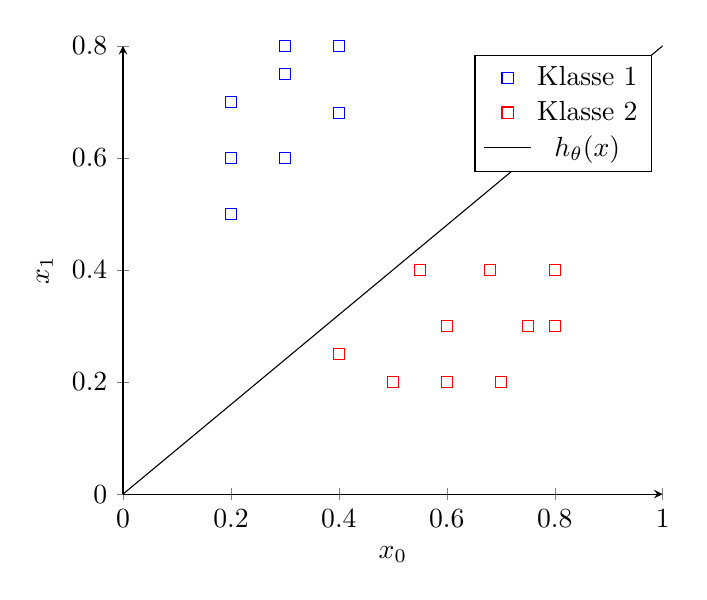
\begin{tikzpicture}
\begin{axis}[
    axis lines = left,
    xlabel = $x_0$,
    ylabel = {$x_1$},
]
\addplot[
    only marks,
    color=blue,
    mark=square,
    ]
    coordinates {
    (0.2,0.7)(0.2,0.5)(0.2,0.6)(0.3,0.8)(0.3,0.6)(0.3,0.75)(0.4,0.8)(0.4,0.68)
    };
\addlegendentry{Klasse 1}
\addplot[
    only marks,
    color=red,
    mark=square,
    ]
    coordinates {
    (0.55,0.4)(0.4,0.25)(0.7,0.2)(0.5,0.2)(0.6,0.2)(0.8,0.3)(0.6,0.3)(0.75,0.3)(0.8,0.4)(0.68,0.4)
    };
\addlegendentry{Klasse 2}
\addplot [
    domain=0:1, 
    samples=100, 
    color=black,
]
{0.8*x};
\addlegendentry{\(h_\theta(x)\)}
\end{axis}
\end{tikzpicture}
\caption{Lineær hypotese skiller datapunktene i to klasser}
\label{figure:separator}
\end{figure}
Separatoren i figur \ref{figure:separator} er en linje i to dimensjoner. En separator i tre dimensjoner vil danne et plan. Å forestille seg en separator i mer enn tre dimensjoner er vanskelig. Heldigvis kan matematikken hjelpe da den ikke bryr seg om våre visuelle begrensninger og fungerer like godt i 128 dimensjoner som i tre. Vi har konkludert med at en lineær modell bør få sjansen til å skille dataeksemplene våre, men hvilken algoritme bør vi benytte? La oss utforske to av de mest brukte og robuste, lineære teknikkene: logistisk regresjon og støttevektormaskiner.

\subsubsection*{Logistisk regresjon}
\begin{equation}
g(x) = \frac{1}{1 + e^{-x}}
\label{eq:sigmoid}
\end{equation}
\begin{figure}[h!]
\centering
\begin{tikzpicture}
\begin{axis}[
    axis lines = center,
    xlabel = $x$,
    ylabel = {$y$},
]
\addplot [
    domain=-5:5, 
    samples=100, 
    color=red,
]
{1 / (1 + e^(-x))};
\end{axis}
\end{tikzpicture}
\caption{Ordinær sigmoidfunksjon}
\label{figure:sigmoid}
\end{figure}
I logistisk regresjon modelleres sannsynlighetene som beskriver ulike utfall av en logistisk sigmoid-funksjon. Denne funksjonen tar en hvilken som helst input-verdi og gir en output-verdi i området \([0,1]\). Likning \ref{eq:sigmoid} og figur \ref{figure:sigmoid} representerer den generelle \emph{sigmoid}-funksjonen. Vi ser at ved større positive x-verdier gir funksjonen et resultat nære 1, mens for større negative verdier gir funksjonen et resultat nære 0.

La oss si vi har to mulige klasser, \(y \in \{0,1\}\). Hvis \( h_\theta(x) \geq  0.5\), gjetter vi at klassen \(y = 1\). Hvis \( h_\theta(x) < 0.5\), gjetter vi \(y = 0\). Når vi nå kombinerer (\ref{eq:hypotese-kompakt}) og (\ref{eq:sigmoid}) får vi den logistiske hypotesen (\ref{eq:logistic}).
\begin{equation}
h_\theta(x) = \frac{1}{1 + e^{-\theta^{T}x}}
\label{eq:logistic}
\end{equation}
Igjen representerer $\theta$ vektingen av egenskapene $x$ i treningsdataene. 
\begin{equation}
J(\theta) = 
    \frac{1}{m} \sum_{i=1}^{m} cost(h_\theta(x^{(i)}), y)
\label{eq:cost}
\end{equation}
(\ref{eq:cost}) viser formelen for logistisk regresjon. Vi ser at $J(\theta)$ er et gjennomsnitt av en kostnadsfunksjon, definert av hypotesen til hvert treningseksempel og den tilhørende korrekte klassen. 
\begin{equation}
    cost(h_\theta(x^{(i)}), y) = \begin{cases}
    -log(h_\theta(x)), & \text{hvis $y=1$}.\\
    -log(1-h_\theta(x), & \text{hvis $y=0$}.
  \end{cases}
  \label{eq:costdetail}
\end{equation}
Kostnadsfunksjonen (\ref{eq:costdetail}) er definert med delt forskrift slik at kostnaden er 0 dersom klassen er 1 og hypotesen er 1, men dersom klassen er 1 og hypotesen går mot 0, går kostnaden mot uendelig. Den delte forskriften gjør at det samme gjelder for det motsatte tilfellet, der kostnaden er lav dersom klassen er 0 og hypotesen gjetter 0, men øker mot uendelig dersom hypotesen går mot 1.
\begin{equation}
\theta_j \leftarrow \theta_j - \alpha \frac{\delta}{\delta\theta_j}J(\theta)
\label{eq:gradient}
\end{equation}
For å tilpasse $\theta$-verdiene er strategien å minimere kostnadsfunksjonen (\ref{eq:costdetail}). Dette gjøres ved å benytte en oppdateringsregel. Regelen oppdaterer egenskapsvektoren $\theta$ ved å trekke fra resultatet fra den partiellderiverte av kostnadsfunksjonen, dempet av en faktor $\alpha$ (\ref{eq:gradient}).

Ettersom den deriverte i et gitt punkt kan sees på som brattheten til kurven i det punktet vil denne oppdateringen tilsvare å stadig ta mindre steg i den retningen som fører mot en lavere verdi. På en to-dimensjonell graf vil det si å følge plottet nedover mot et bunnpunkt, men algoritmen fungerer på samme vis i høyere dimensjoner. Denne oppdateringsregelen kalles "gradient descent" og brukes i maskinlæringsalgoritmer for å finne minimumsverdier.

Etter at $\theta$-verdiene er tilpasset av treningsdata kan modellen gjette hvilken klasse et nytt datapunkt tilhører ved å benytte (\ref{eq:logistic}). For å lære å skille mellom mer enn to ulike klasser benyttes strategien "en-mot-resten". For hver klasse trenes det en egen hypotese som best mulig skiller mellom denne klassen og alle de andre. Når ny data kommer inn til det trente systemet velges den hypotesen som gir den høyeste sannsynligheten for en viss klassifisering og dermed er mest sikker på å ha funnet det riktige svaret. I tillegg til å fortelle hvilken klasse dataeksempelet tilhører kan logistisk regresjon fortelle hvor sikker klassifiseringen er. Dette er en god egenskap som støttevektormaskiner mangler.

\subsubsection*{Støttevektormaskiner (SVM)}
Støttevektormaskiner er en annen gruppe med maskinlæringsalgoritmer som kan brukes til å løse klassifiseringsproblemer. De er kjent for å være effektive i problemområder med mange dimensjoner og kan oppnå gode resultater selv når antallet dimensjoner er høyere enn antall treningseksempler. De bruker mindre plass i minnet enn andre tilnærminger og kan tilpasses til å løse en rekke forskjellige problemer. To ulemper med SVM-er er at de ikke tilbyr direkte estimater på hvor sikker klassifiseringen er og at de, som logistisk regresjon, i utgangspunktet bare kan skille mellom to klasser.

I figur \ref{figure:separator} så vi en lineær hypotese som tydelig delte datapunktene i to klasser. I figuren ligger den separerende hypotesen nærmere datapunktene for klasse 2. Dette er vist som et resultat av at det er flere treningseksempler av denne typen og dermed har den lineære metoden produsert en hypotese som ligger nærmere disse datapunktene. Vi kan også forstå at det må være et uendelig antall forskjellige hypoteser som kan dele datapunktene, men at en hypotese som ligger midt mellom de to klassene av datapunkter vil være den mest robuste. Støttevektormaskiner benytter nettopp denne intuisjonen for å finne en optimal hypotese. Med støttevektormaskiner kalles separatoren et hyperplan som kan danne skiller i høydimensjonelle rom. En optimal deling oppnås av det hyperplanet som har den største avstanden til det nærmeste datapunktet hos hver klasse. Denne strategien om å finne den største marginen mellom klassene senker generelt klassifikatorens feilaktighet. Figur \ref{figure:svm} viser et slikt optimalt hyperplan som befinner seg der hvor marginene til hver klasse er maksimal og like stor.
\begin{figure}[h!]
\centering
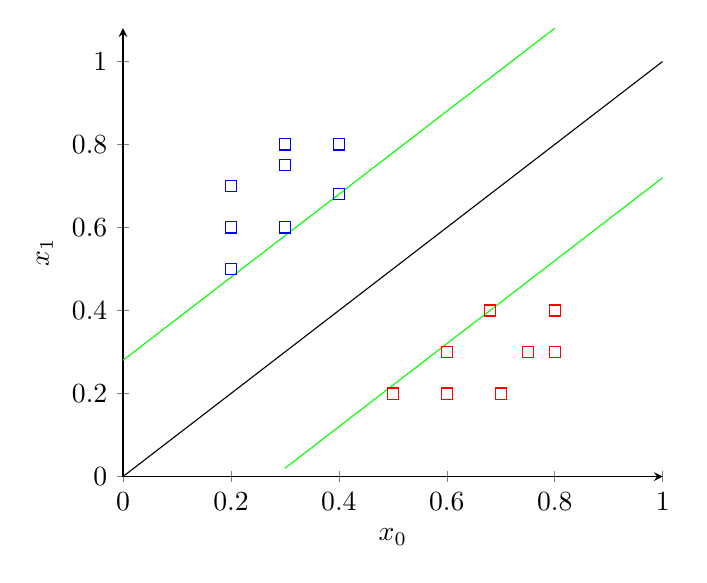
\begin{tikzpicture}
\begin{axis}[
    axis lines = left,
    xlabel = $x_0$,
    ylabel = {$x_1$},
]
\addplot[
    only marks,
    color=blue,
    mark=square,
    ]
    coordinates {
    (0.2,0.7)(0.2,0.5)(0.2,0.6)(0.3,0.8)(0.3,0.6)(0.3,0.75)(0.4,0.8)(0.4,0.68)
    };
\addplot[
    only marks,
    color=red,
    mark=square,
    ]
    coordinates {
    (0.7,0.2)(0.5,0.2)(0.6,0.2)(0.8,0.3)(0.6,0.3)(0.75,0.3)(0.8,0.4)(0.68,0.4)
    };
\addplot [
    domain=0:0.8, 
    samples=100, 
    color=green,
]
{x + 0.28};
\addplot [
    domain=0.3:1, 
    samples=100, 
    color=green,
]
{x - 0.28};
\addplot [
    domain=0:1, 
    samples=100, 
    color=black,
]
{x};
\end{axis}
\end{tikzpicture}
\caption{Det optimale hyperplanet i svart og de to støttevektorene i grønt}
\label{figure:svm}
\end{figure}
Treningen av støttevektormaskiner følger det samme mønsteret som logistisk regresjon, men skiller seg på å ha en annen hypotese og kostnadsfunksjon. Hypotesen er det lineære indreproduktet vi så fra introduksjonen om klassifisering (\ref{eq:hypotese-kompakt}). Kostnadsfunksjonen er enklest forstått gjennom et plot.
\begin{figure}[h!]
\begin{subfigure}{0.5\textwidth}
\centering
\begin{tikzpicture}
\begin{axis}[
    axis lines = center,
    xlabel = $\theta^{T}x$,
    xmin=-2, xmax=2,
    ymin=0, ymax=5,
]
\addplot [
    domain=-2:2, 
    samples=100, 
    color=red,
]
{1 + x};
\addplot [
    domain=-2:-1, 
    samples=100, 
    color=red,
]
{0};
\legend{$cost_0(\theta^{T}x)$}
\end{axis}
\end{tikzpicture}
\end{subfigure}
\begin{subfigure}{0.5\textwidth}
\centering
\begin{tikzpicture}
\begin{axis}[
    axis lines = center,
    xlabel = $\theta^{T}x$,
    xmin=-2, xmax=2,
    ymin=0, ymax=5,
]
%\addlegendentry{$cost_0(\theta^{T}x)$}
\addplot [
    domain=-2:2, 
    samples=100, 
    color=blue,
]
{1 - x};
\addplot [
    domain=1:2, 
    samples=100, 
    color=blue,
]
{0};
\legend{$cost_1(\theta^{T}x)$}
\end{axis}
\end{tikzpicture}
\end{subfigure}
\caption{Støttevektormaskinens kostnadsfunksjoner}
\label{figure:svmcost}
\end{figure}
(\ref{figure:svmcost}) viser de to kostnadsfunksjonene. Dersom klassen $y=1$ ønsker vi at hypotesen $\theta^{T}x \geq 1$. Dersom klassen $y=0$ ønsker vi at hypotesen $\theta^{T}x \leq -1$

Treningen består dermed igjen av å minimere (\ref{eq:svmcost}) med den samme oppdateringsregelen som for logistisk regresjon (\ref{eq:gradient}), men med en ekstra, justerbar parameter $C$ som avgjør hvor mye man ønsker å unngå å feilklassifiere hvert treningseksempel. Med en stor $C$-verdi vil optimaliseringen velge et hyperplan med mindre marginer dersom dette hyperplanet gjør en bedre jobb på å få alle treningsdataene klassifisert riktig. En lav $C$-verdi lar optimaliseringen finne et hyperplan med større marginer, selv dersom dette hyperplanet feilklassifiserer flere datapunkt.
\begin{equation}
J(\theta) = 
    C \sum_{i=1}^{m} y^{(i)}cost_1(h_\theta(x^{(i)})) + (1-y^{(i)})cost_0(h_\theta(x^{(i)}))
\label{eq:svmcost}
\end{equation}
Den typen SVM vi har presentert her er en såkalt lineær SVM eller en SVM uten kjerne. Ved å benytte et såkalt "kernel trick" kan SVM-er også modellere ikke-lineære funksjoner. Dette gjør SVM-er svært fleksible til å håndtere ulike data. I dette prosjekt er vi kun interessert i de lineære modellene. For å håndtere klassifisering av flere klasser benyttes gjerne den samme "en-mot-resten"-strategien som i logistisk regresjon. Denne ender altså opp med å trene $n$ klassemodeller og modellen med det beste resultatet benyttes.

\subsection{Brukergrensesnitt}
{\color{blue}Noe om disse to reffene}\citet{levold07} \citet{victor06}
Programvare eksisterer for å hjelpe folk med å lære, å skape eller å kommunisere. \emph{Informasjonsprogramvare} hjelper folk med å lære. En person bruker informasjonsprogramvare for å konstruere og manipulere en intern representasjon av informasjonen. \emph{Manipulasjonsprogramvare} hjelper folk med å skape. En person bruker manipulasjonsprogramvare for å skap og manipulere en virtuell modell representert på datamaskin. Denne typen programvare kan bli forstått som et virtuelt verktøy, som en malingskost eller skrivemaskin, som benyttes som et grensesnitt mellom skaperen og sluttproduktet. \emph{Kommunikasjonsprogramvare} hjelper folk med å kommunisere. En person bruker kommunikasjonsprogramvare for å skape og manipulere en intern modell som er delt, forstått og synkronisert mellom flere mennesker. Kommunikasjon kan sees på som å lage et svar på tillært informasjon. Den eksterne modellen en bruker kommuniserer er den interne modellen brukeren har lært.

Brukere i smarte hjem trenger programvare til å gi kommandoer til hjemmet, som å skru på lyset i et rom eller låse utgangsdøra, og til å lære om hjemmets tilstand, som å se temperatur, status på oppvaskmaskina eller om det mangler matvarer i kjøleskapet. Hvordan kan man effektivt og naturlig kan gi kommandoer til hjemmet? Hvordan kan relevant informasjon om hjemmet kan presenteres for brukeren?

{\color{red}Diskuter om direkte manipulasjon er best for brukergrensesnitt eller om brukergrensesnitt skal tilpasse seg dynamisk og forsøke å hjelpe brukeren. MER.}\citet{directmanipulation}

I introduksjonen definerte jeg \emph{IUI} til å være grensesnitt mellom mennesker og datamaskiner med et mål om å være mer effektive og mer naturlige i bruk. \citet{Kaufmann98} påpeker at dette oppnås gjennom å representere, resonnere og handle på modeller av brukeren, domenet, oppgaven, diskusjonen og mediumet. \emph{IUI} er en del av \emph{HCI}, ergonomikk, kognitiv vitenskap og \emph{AI}.

Målet til HCI er å gjøre datamaskiner mer hjelpsomme og enklere å bruke. \citet{Lieberman09} skriver om hvordan HCI og AI er relaterte og hvordan de bør samarbeide og kan lære av hverandre for å løse målene våre. Det må insses at det er "trade-offs" mellom systemets pålitelighet og grad av konsekvens, og systemets evne til å forstå hva brukeren øsnker og å tilby hjelp. Lieberman påpeker videre at avanserte brukergrensesnitt muligens trenger "tutorials" for å gjøre brukeren komfortable. Brukerens behov forandrer seg stadig så å ta utgangspunkt i et dynamisk system gir fleksibilitet til å håndtere framtidige forandringer. HCI har investert mye i forskning på modeller som \emph{GOMS} eller \emph{key-stroke}, for å modellere sammenhengene mellom oppgaver og operasjonene som trengs for å fullføre dem i et gitt grensesnitt. Disse modellene hjelper med å evaluere effektiviteten i brukergrensesnittene. Å introdusere intelligens i systemene kan la brukere unngå utførelsen av en rekke operasjoner for å nå et mål. Brukeren kan i stedet angi et overordnet mål og det er så opp til systemet å finne ut hva som må gjøres for å oppnå målet.

\subsubsection*{Smarttelefoner og andre touch-skjermer}
Touchskjermer i form av smarttelefoner og nettbrett er nå vidspredte og populære. Dette er dermed en interaksjonsform folk bør være komfortable med å styre funksjonalitet i hjemmet. At nesten alle har smarttelefoner med seg til enhver tid gjør også at muligheten til informasjon om og styring av hjemmet alltid er tilgjengelig.

\citet{koskela04} undersøkte forskjellige brukergrensesnitt for å styre smarte hjem. De evaluerte bruken av en pc, en tv med fjernkontroll og en mobiltelefon. Resultatene viste at en pc fungerte best som en sentral enhet for å kontrollere aktiviteter som kan planlegges eller bestemmes på forhånd. Dette gjaldt å sette opp automatiseringer, slik som at gardinene skal trekkes for og at lysene skrus på til et visst tidspunkt. Mobiltelefonen ble funnet til å være det beste alternativet for direkte kontroll. Denne studien ble gjort i 2004 og resultatene kan derfor antas å være noe daterte, men resultatet om at en bærbar, mobil enhet var det beste for å direkte kontrollere omgivelsene er nyttig. Dagens smarttelefoner er selvfølgelig kapable til mye mer enn mobiltelefonen fra 2004 og dermed er smarttelefoner og andre touch-skjermer sannsynligvis et godt alternativ for å tilby interaksjon med hjemmet.

\subsubsection*{Omgivelsesskjermer}
I kapitellet om smarte hjem pratet jeg om \emph{AmI} og teknologi innbakt i miljøet. En teknologi det forskes på er omgivende skjermer. Informasjonskilder, andre mennesker og omgivelsene skal kunne sees og interageres med når det er behov for det. Å ha informasjonskilder tilgjengelig forskjellige steder i hjemmeomgivelsene kan gi nye muligheter for samarbeid mellom mennesker i aktiviteter som omhandler både lek og arbeid.

Forskjellige interaksjonssoner beskrives av \citet{streitz05}. De omtaler interaksjonssonene omgivende, notifikasjon og interaksjon. \emph{Proxemics} foreslås av \citet{greenberg11} som en tilnærming for å gi enheter en mer naturlig oppførsel. De stipulerer at brukere naturlig forventer at når enhetene deres nærmer seg andre enheter eller gjenstander i omgivelsene, øker tilkoblingen og interaksjonsmulighetene forbedres. Bruken av soner gir mulighet til å tilby forskjellige visninger og interaksjoner basert på avstand. Greenberg et al. omtaler fem målbare dimensjoner av \emph{proxemics}: \emph{Avstanden} mellom enheter og brukere passer godt inn med interaksjonssonene som er definert. \emph{Retning} gir et mål på vinkelen mellom enheter og brukere. Det finnes allerede enheter som gjør bruk av retning, for eksempel ved å skru seg av når folk ikke ser på dem. \emph{Bevegelse} omfatter forandring i distanse over tid. \emph{Identitet} beskriver en enhet i et gitt detaljnivå. \emph{Plassering} beskriver posisjonen til enheten, for eksempel i hvilket rom og hva konteksten rundt rommet er. \emph{Proxemics} kan i sin helhet være med på å tilby en mer naturlig interaksjon med enhetene våre og kan kanskje være det neste steget for utviklingen av interaksjonsapplikasjoner.

\subsubsection*{Gester}
Interaksjon med gester er et forsøk på å tilby en mer naturlig interaksjon med datamaskinen. Kroppsspråket er tross alt en stor del av mellommenneskelig kommunikasjon, så hvorfor ikke forsøke å utvide det til kommunikasjon mellom menneske og maskin.
De fleste prosjektene som utforsker bruker av gester benytter kameraer som måler farger og dybde, samt avanserte datasynsalgoritmer for å gjøre mening av dataene. Sammen kan disse prosessere informasjonen og danne grunnlaget for et system som kan gjenkjenne kompliserte gester.

Et eksempel omtales av \citet{homeos}. Dette prosjektet ble utført med bruk av \emph{Kinect}-kameraet\footnote{kinecturl} til å forstå gester.

{\color{red}Her trengs det et par ekstra eksempler fra artiklene.}

\subsubsection*{Multimodalitet}
Multimodalitet i forbindelse med datasystemer betyr å forbedre forståelsen gjennom en kombinasjon av flere input-kanaler. Meningen er å forbedre systemets nøyaktighet i å oppdage og forstå input-signaler, kanskje spesielt når dataene kommer på forskjellige og ikke-overlappende former. \citet{placelab05} beskriver \emph{Placelab}-prosjektet som et bra eksempel på å kombinere video og audio for å bedre nøyaktigheten i å detektere menneskelig aktivitet. Mange prosjekter gjør bruk av kombinasjoner av diverse sensorteknologier for å danne et rikere tilstandsbilde og for å forbedre nøyaktigheten. \citet{desilva12} nevner et prosjekt der en robot følger et menneske gjennom multimodale teknikker. Roboten har en visuell input og er trent gjennom maskinlæring til å skille hudfarge fra omgivelsene og dermed identifisere mennesket. I tillegg benytter roboten seg av en sonarskanner samt taktile sensorer for å beregne avstanden til mennesket.

\citet{quickset97} beskriver \emph{QuickSet}, et multimodalt system som ..{\color{red}infos}.

{\color{red}integrating simultaneous input, multimodal interfaces: survey, mmhci: survey}

\subsubsection*{Brain Interfaces, Blikk \& Annet}
Mennesker bruker kroppen sin som et grensesnitt til verden. Dette systemet har utviklet seg over millioner av år og fungerer utmerket. Brukergrensesnitt til datamaskiner er et helt nytt konsept. Dersom det er problemer mellom kroppene våre og datamaskiner, ville det ikke vært mest naturlig å sette spørsmål ved datamaskinen, ikke kroppen? Datamaskinene bør vel tilpasses til å best mulig bruke våre kropper, i stedet for å forbigå kroppen totalt. Vi er allerede i ferd med å miste kroppene våre. Vi sitter stille mesteparten av dagen, både gjennom arbeid, reise og fritid. Jeg er ikke sikker på om brain interfaces er hva vi ønsker for framtiden.

Dette er teknologi som er verdt å utforske for å hjelpe funksjonshemmede. Det er også interessant å se hva datamaskinene kan lære om følelsene våre ved å lytte på hjerneaktiviteten. Men jeg tror ikke dette er et aktuelt og verdifullt brukergrensesnitt å utforske for fremdeles friske mennesker.

{\color{red}kort om blikk, vep, og annet fra iui}

\subsubsection*{Dynamiske brukergrensesnitt}
I \ref{ch:smartehjem} så vi på hva brukerene ønsker seg. Noen av disse ønskene kan være vanskelig å implementere uten å bryte andre ønsker, som at systemet skal forstå konteksten i omgivelsene uten å være overvåkende. Det viktigste for de spurte gruppene var å selv være i kontroll av et systemet som var enkelt å bruke og som ga muligheter til å styre diverse deler av huset, inkludert elektriske apparater, hvitevarer, hjemmeunderholdning, lys og varme. Alt i alt er det kanskje viktigere for vanlige brukere at det tilbys gode styringsmuligheter, enn at systemet er proaktivt og forsøker å forstå hva brukeren ønsker?

\citet{rogers06} påpeker at forskningsmiljøet har møtt spesielt store problemer med den store variasjon i hva folk gjør, hvilke motiver de har, når de gjør det og hvordan de gjør det. Konteksten rundt folks dagligdagse liv er svært subtil. Dette gjør det vanskelig, om ikke umulig, å implementere kontekst slik at det kan gjøres nyttige spådommer om hva mennesker føler, hva de ønsker eller hva de trenger i et gitt øyeblikk. Det finnes også etiske og sosiale bekymringer.

Rogers argumenterer for et skifte fra proaktiv databehandling to proaktiv mennesker. Allestedsnærværende teknologier bør designes slik at brukere kan interagere med dem mer aktivt. Mennesker, i stedet for maskiner, bør ta initiativet til å være konstruktive, kreative og engasjere i interaksjoner. I stedet for å pakke omgivelsene med all slags forsvinnende teknologi, bør vi tenke på teknologien som et sett med verktøy og overflater, som er mobile og tilrettelegger for samarbeid. Informasjonskilder, andre mennesker og omgivelsene kan sees og interageres med når det er behov for det. Vi må få tilbake gleden med interaksjon på innovative måter.

Interaktiv media gir brukere personlig tilgang til informasjon. I designet av programvare-basert media opplever designeren at det er umulig å designe en løsning til et spesifikt problem og at han i stedet må representere en måte å designe programvare på som kan generere løsninger i "run-time". \citet{ishizaki96} presenterer \emph{maDes}, en arkitektur som oppfordrer designere til å anse et designproblem som en kontinuerlig strøm, framfor en samling diskret problemer, og en designløsning som en entitet generert av den dynamiske aktiviteten til designelementer, framfor et sett med designelementer med faste attributter. \emph{maDes} modellerer en designløsning som et system bestående av en samling av mindre designsystemer. Hvert system er en \emph{designagent} og er ansvarlig for å presentere en bestemt type informasjon. En designagent kan tilpasse hvordan informasjon vises ut fra forandring i kontekst og gjennom samarbeidet med andre designagenter.

\subsubsection*{Tale}
Å gi datamaskinen evnen til å forstå og utøve tale er en av teknikkene fra AI som har hatt kommersiell suksess. Talegjenkjenning benyttes daglig av brukere verden over for å gi navigasjonsinstrukser til bilene sine, gjøre søk på nettet eller å skrive gjennom diktasjon. Tale er en attraktivt interaksjonsform i alle tilfeller der brukeren kan ha bruk for å gjøre andre ting med hendene, eller der han ikke har muligheten til å bruke dem.

Det er ingen enkel oppgave å gjenkjenne tale. Lydene brukeren lager inneholder ofte støy og det finnes en rekke setninger som høres like ut når de sies fort. Når vi skriver setninger er det mellomrom mellom ordene, men i tale er det setninger som uttales uten pause mellom ordene. Det er også mange ord som uttales likt, men skrives forskjellig og har forskjellig betydning avhengig av kontekst.

\citet{russellnorvig10} omtaler talegjenkjenning som å være identifikasjonen av en sekvens av ord ut i fra et akustisk signal.
Talegjenkjenning handler om å finne den mest sannsynlige sekvensen av ord. Denne mest sannsynlige sekvensen kan kalkuleres ved bruk av Bayes' regel:

{\color{red}bayes} argmax P(word|sound) er lik argmax P(sound|word)P(word)
P(sound|word) er en akustitisk modell; en beskrivelse av lydene til ord. P(word) er språkmodellen, som sier noe om den foregående sannsynligheten til hver uttale. For eksempel kan språkmodellen si at "Spise iskrem" er 1000 ganger så sannsynlig som "Grise iskrem".

De fleste talegjenkjenningssystemene i dag benytter en språkmodell etter \emph{Markov-antakelsen}, altså at den nåværende tilstanden, \emph{Word1}, avhenger kun av et fiksert antall foregående tilstander, og \emph{Word1} er representert som en enkelt tilfeldig variabel bestpende av et begrenset sett med verdier, hvilket gjør den til en \emph{Hidden Markov Model (HMM)}. Altså kan talegjenkjenning løses ved å anvende \emph{HMM}-metodologien.

Carnegie Mellon University påpeker at virkeligheten med tale ikke er så enkelt som man skulle tro. Intuisjonen er at tale er bygget opp av ord, og at hvert ord består av fonemer. I virkeligheten er det desverre svært annerledes. Tale er en dynamisk prosess uten klare skiller mellom ulike deler. De moderne måtene å beskrive tale på er i større eller mindre grad basert på sannsynligheter. Denne måten å se situasjonen på lar oss forstå at talegjenkjenning aldri vil være 100\% korrekt\footnote{http://cmusphinx.sourceforge.net/wiki/tutorialconcepts}.

Tale er en kontinuerlig strøm av audio der relativt stabile tilstander blander seg med dynamiske tilstander. I denne strømmen av tilstander kan man forsøke å definere klasser av lyder, kalt fonemer. De akustiske egenskapene til bølgeformen til et fonem kan variere kraftig avhengig av faktorer som omgivelseslyder, hvem som taler og hvordan denne kilden taler. Disse variasjonene kan gjøre at fonemer oppfattes svært annerledes ut enn det de skulle representere. 
En strategi for å hjelpe mot disse problemene er å innse at de viktigste datapunktene er i overgangene mellom ord. Utviklere benytter ofte tre regioner i strømmen for å gjenkjenne et ord: den første delen avhenger av det foregående fonemet, midtpartiet er relativt stabilt, og den tredje delen avhenger av det følgende fonemet. Fonemer bygger subord-enheter, som stavelser. Stavelser kan være nyttige å modellere etter og de er kjent som "reduction-stable entities". Når tale utføres raskt vil fonemer ofte være annerledes, men stavelser forblir de samme. Flere subord danner ord. Ord er viktig i talegjenkjenning fordi de begrenser kombinasjonen av fonemer. Dersom det er 40 fonemer og et gjennomsnittlig ord har 7 fonemer finnes det 40 opphøyd i 7 mulige ord. Heldigvis benytter de fleste mennesker omtrent 10000 ord til daglig, hvilket gjør talegjenkjenning mer håndterlig.

Ord, sammen med andre ikke-lingvistiske lyder (som pust, hoste, pauselyder), danner ytringer. Ytringer er separate lyder mellom pauser. 

Den vanlige måten å gjenkjenne tale på er følgende: man mottar en bølgeform, splitter den inn i ytringer delt av stillhet og forsøker så å gjenkjenne hva som blir sagt i hver ytring. For å gjøre dette tar vi alle mulige kombinasjoner av ord og forsøker å matche dem med lyden. Vi velger så den kombinasjonen som passer best.

Tale modelleres gjerne med en Hidden Markov Model (HMM). Modellen beskriver en sekvens av tilstander der overgangen er gitt av en sannsynlighet. Det er en generell modell som kan beskrive alle sekvensielle prosesser og den har vist seg å være spesielt praktisk for å dekode tale.

Tre modeller benyttes i talegjenkjenning for å matche ord med lyd. En akustisk modell, en ordbok og en språkmodell. Den akustiske modellen holder akustiske egenskaper for kombinasjoner av fonemer. En enkel fonetisk ordbok knytter ord med fonemer. Denne naive varianten er ikke veldig effektiv ettersom den ikke tar større hensyn til forskjellige uttaler, men den fungerer som regel i praksis. Maskinlæring kan benyttes her for å lære langt mer nyanserte sammenhenger. En språkmodell brukes for å innsnevre søket etter det passende ordet. Den definerer hvilke ord som kan følge etter det foregående gjenkjente ordet og hjelper dermed med å fjerne ord som ikke er sannsynlige. De fleste språkmodeller er n-gram modeller, som inneholder statistikk over ord-sekvenser, eller finite-state-modeller, som definerer talesekvenser av finite-state-automation med vekting. For å oppnå en god presisjon må språkmodellen utføre en god jobb på å begrense søkeområdet for mulige ord. Den må altså være svært god på å gjette det neste ordet. En språkmodell begrenser som regel vokabularet til ordene den inneholder. Dette skaper problemer med navn-gjenkjenning. Derfor kan en språkmodell også inneholde mindre deler, som subord eller til og med fonemer. Søkeområdet øker dersom disse introduseres og leder som regel til svakere presisjon enn med en ord-basert språkmodell.



